\documentclass{article}
\usepackage[utf8]{inputenc}
\usepackage[margin=1in]{geometry} % set the margins to 1in all around
\setlength\parindent{0pt} % don't automatically indent text

\usepackage{csquotes} % enquote
\usepackage{enumerate}
\usepackage{multirow, tabularx} % multirow

\usepackage{amsmath, amssymb, amsfonts}
\usepackage{physics} % abs

\usepackage{listings}
% some basic styling for code snippets
\lstset{basicstyle=\footnotesize\ttfamily}

\usepackage{graphicx}
\graphicspath{{./}} % get images from this directory

\newcommand{\R}{\mathbb{R}}
\newcommand{\Z}{\mathbb{Z}}

\begin{document}
\section*{Overview}
In this document we'll cover the basics of latex, as well as some more advanced
math features I expect to use in the assignments. Some of the stuff I'll cover
is:
\begin{itemize}
\item basic latex stuff like font formatting, lists, and tables
\item math stuff including matrices, math environments, and math symbols
\item including images and code in your document
\end{itemize}

\section*{Basics}
If you're reading the source code, you've probably already seen some of the
commands and environments I'll be going over in this section - though maybe
you're already familiar with them. And in fact everything in this section, you
can probably find better reference for on Overleaf, but I'm including it anyway
because it may be useful to have useful things all in one place.~\\

Before getting into things, it's probably important to note that I'll be listing
a bunch of commands by their name, but just know that a command in latex might
look something like \textbackslash command\{argument\}. You can see many
examples of this in the source for this document.

\subsection*{Font Formatting}
Just some really basic stuff: 
\begin{itemize}
\item you can write \textbf{bold text} with \lstinline{textbf}
\item \textit{italics} are written with \lstinline{textit}
\item \underline{underline} your text with \lstinline{underline}
\item a one that's a little less known is \enquote{proper quotations} using
      \lstinline{enquote} from the package \lstinline{csquotes}. If you use
      regular "quotation marks" they'll end up both pointing the same way :-/
\end{itemize}

\subsection*{Lists}
Lists in latex can be very simple, but they can also be complex if you want
them to be. One important note is that lists in latex are probably the first
\textit{environment} you'll come across. An environment is essentially something
you need to \lstinline{begin} and \lstinline{end}, unlike the commands you've
seen so far. You can see examples of all of this in action in the source
document.

\begin{itemize}
\item \textbf{unordered} lists can be made via the \lstinline{itemize}
      environment
\item all list environments require you to give them \enquote{items} like the
      two here
\end{itemize}

\begin{enumerate}[1.]
\item \textbf{ordered} lists use the \lstinline{enumerate} environment.

\item enumerate is actually defined in more than one package. The simplest
      package to use is \lstinline{enumerate}, but if you're not satisfied
      with it's capabilities, a more flexible but also less approachable
      package \lstinline{enumitem} also defines the enumerate environment

\item some environments like \lstinline{enumerate} also take arguments in
      square braces
      \begin{enumerate}[(a)]
      \item in the enumerate package you can specify what symbols to use for
            your ordering, as well as other frills like ending with a period
            or parentheses.
      \item you can also nest any list in any sort of environment
      \end{enumerate}
      \begin{itemize}
      \item even mix different types of list environments
      \end{itemize}
\end{enumerate}

\subsection*{Tables}
Tables are often very useful in latex
\begin{tabular}{cc}
a & b\\
c & d\\
\end{tabular}

\begin{itemize}
\item This simple 2x2 table is made with the \lstinline{tabular} environment.
\item The tabular environment takes arguments in curly braces (as opposed to
      square braces like with list environments).
\item The arguments to the tabular environment tell latex how many columns to
      make and how to justify each colum

      So \textbf{lcr} as arguments tells the table to make three columns that
      are left, center, and right-justified respectively.

\item you can also give your tables vertical and horizontal bars. for example,
      my favorite table format looks like this

      \begin{tabular}{c|cc}
        & a & b \\
      \hline
      c & 1 & 2 \\
      d & 3 & 4 \\
      \end{tabular}

      you can see in the source code that the vertical bar was specified in the
      arguments to the tabular environment, while the horizontal bar was it's
      own line in the table, using the no-argument command \lstinline{hline}.

\item The last thing I want to mention about tables is the ability to combine
      cells. This can be done using the \lstinline{multirow} and
      \lstinline{multicolumn} commands.

      In this example, both take three arguments in separate curly braces:
      the number of cells
      to span, the justification and border info for multicolumn - and cell
      width infor for multirow, and finally the content of the cell

      \begin{tabular}{c|cc}
        & \multicolumn{2}{c}{span two columns}\\
        \hline
        \multirow{2}{*}{span two rows}
        & 1 & 2\\
        & 3 & 4
      \end{tabular}

      Although the multirow command requires the \lstinline{multirow} and
      \lstinline{tabularx} packages.
\end{itemize}

\subsection*{Sections}
Finally, I'll breifly mention sections and subsections. As you can see in the
source, I've been using these throughout to create headers for sections and
subsections just as you might expect. One important note is that I use an
asterisk after the command name to tell latex that I don't want the sections
to be ordered. This is a personal preference and if you do want ordered
sections just leave out the asterisk

\section{An example of an ordered Section}
\subsection{And an ordered subsection}

As a last word I'll also mention the command \lstinline{newpage} which - as
you might guess - inserts a page break. This is very useful for organizing your
document as I'll do now to give a clean break to the next section.

\newpage
\section*{Some mathy things}
While latex has some pretty useful stuff for formatting and whatnot, the meat
of why people use latex is usually to write complex mathematical expressions
that are more difficult to work with in word processors. I'll go over some of
the best ways I know of to deal with these tricky expressions in latex.

\subsection*{Math symbols}
The first thing you need to do is make sure you're using the appropriate
packages. Most math symbols you'll use are defined in \lstinline{amsmath},
but you may end up wanting fancy math symbols from \lstinline{amssymb} and
\lstinline{amsfonts} like $\not\subseteq$ or $\mathcal{F}.$~\\

Probaby the easiest way to show different math symbols is with a table, but
before I get to that, a few math things that don't really fit in a table:
\begin{itemize}
\item superscripts and subscripts like $x^2$ and $a_i$ are acheived by using
      the carrot symbol and the underscore respectively. Though if you want
      more than one character in your super/sub-scripts you'll need to enclose
      it in curly braces like $2^{3n}$ or $b_{ij}$

\item if you want to use bold text in a math environment you should use
      \lstinline{mathbf} instead of \lstinline{textbf}
\end{itemize}

Now, some math symbols~\\

\begin{tabular}{c|lcc|l}
symbol & command & & symbol & command\\
\hline
 & & & & \\
$\frac{a}{b}$ & frac with two arguments &
              & ${a\choose b}$ & \{a \textbackslash choose b\}\\
 & & & & \\
$\int_a^b$ & int with sub/super-scripts &
           & $P(A \mid B)$ & mid (the vertical bar) \\
 & & & & \\
$\sum_{i=0}^n$ & sum with sub/super-scripts &
               & $P(\overline{X})$ & overline with one argument \\
 & & & & \\
$\sqrt{x}$ & sqrt with one argument & & & \\
\end{tabular}

~\\

All the greek letters are basically just their english spellings. However, I
typically like $\varnothing$ and $\varepsilon$ over $\emptyset$ and $\epsilon$.
There are also many fancy math characters available from the 
mathbb and mathcal commands.
I use fields like $\mathbb{R}$ so often that I usually define a new command
for them like $\R$ as you can see in the preamble (the stuff before begin
document)

\subsection*{Matrices and piecewise functions}
Matrices in latex are their own environment - however they're very similar
to the tabular environment in that you separate rows by newlines and columns
by ampersands. Depending on the delimiters you prefer, you can
use \lstinline{pmatrix} for parenthesis, \lstinline{bmatrix} for squar brackets,
and \lstinline{Bmatrix} for curly brackets. For example

\begin{equation*}
\begin{pmatrix} a & b \\ c & d \end{pmatrix}
\begin{bmatrix} a & b \\ c & d \end{bmatrix}
\begin{Bmatrix} a & b \\ c & d \end{Bmatrix}
\end{equation*}

Another vaguely similar command is for piecewise functions and it's
\lstinline{cases}

\begin{equation*}
\abs{x} = \begin{cases} x & \text{if } x \geq 0 \\
                       -x & \text{if } x < 0
          \end{cases}
\end{equation*}

\newpage
\subsection*{Math environments}
One of the first things many people learn in latex is to use the dollar sign
for inline math like $e^{i\pi} = -1$ and to use double dollar signs for a
more spacious math environment like

$$
e^{ix} = \cos(x) + i\sin(x)
$$

However, as you get into more complicated expressions the double dollar sign
environment actually becomes a lot harder to work with and it's usually a better
idea to use the \lstinline{equation} or \lstinline{align} environments, for
instance

\begin{equation*}
e^{ix} = \sum_{n=0}^{\infty} \frac{(-1)^n}{(2n)!}x^{2n}
                          + i\frac{(-1)^n}{(2n+1)!}x^{2n+1}
\end{equation*}

or here's an aligned equation involving matrices

\begin{align*}
\mathbf{U\Sigma V^T} &= \begin{pmatrix}
                     & & & &\\
                     & & & &\\
                     \mathbf{u_1} & \ldots & \mathbf{u_r}
                                  & \ldots & \mathbf{u_m}\\
                     & & & &\\
                     & & & &\\
                     \end{pmatrix}
                     \begin{pmatrix}
                     \sigma_1 & & & &\\
                     & \ddots & & &\\
                     & & \sigma_r & &\\
                     & & & &\\
                     \end{pmatrix}
                     \begin{pmatrix}
                     & & \mathbf{v_1^T} & & \\
                     & & \vdots & & \\
                     & & \mathbf{v_r^T} & & \\
                     & & \vdots & & \\
                     & & \mathbf{v_n^T} & & \\
                     \end{pmatrix}\\
                  &= \mathbf{u_1}\sigma_1\mathbf{v_1^T}
                   + \ldots + \mathbf{u_r}\sigma_r\mathbf{v_r^T}
\end{align*}

\newpage
\section*{Dealing with images, plots and code}

\subsection*{Including code}
You may have seen me use \lstinline{lstinline} a lot - and you've probably
guessed that it makes inline code snippets. However you can also include code
from a file using \lstinline{lstinputlisting}.

\lstinputlisting[language=Python]{sample.py}

Both of these commands require you to use the \lstinline{listings} package.
You can also customize the style of the code snippets. You can see I did a
basic styling in the preamble.

\subsection*{Including images}
Of course, you can also have images in your document. This can be done using
the command \lstinline{includegraphics} from the \lstinline{graphicx} package.
With the \lstinline{graphicx} package, you can specify a directory that you've
saved your image files in, so you can include them just by their name.~\\

You can also specify some arguments like width in square braces before the name
of the image. Sepcifying width will scale the image. The \lstinline{textwidth}
macro is a useful constant for this that gives the width of the page.
Here are the two images generated from the python code included above.

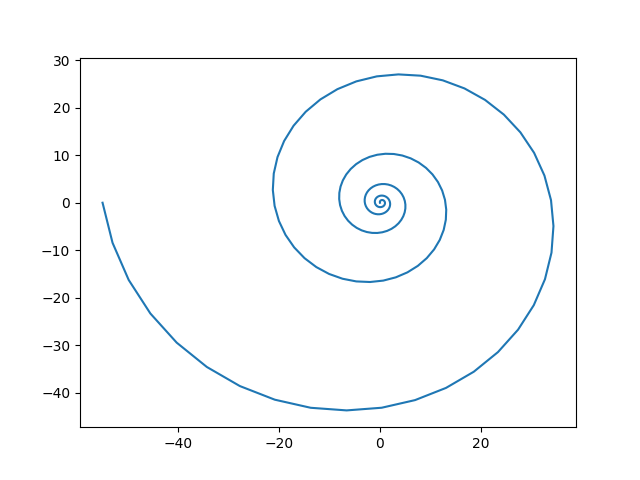
\includegraphics[width=0.5\textwidth]{fibonacci-negative-n.png}
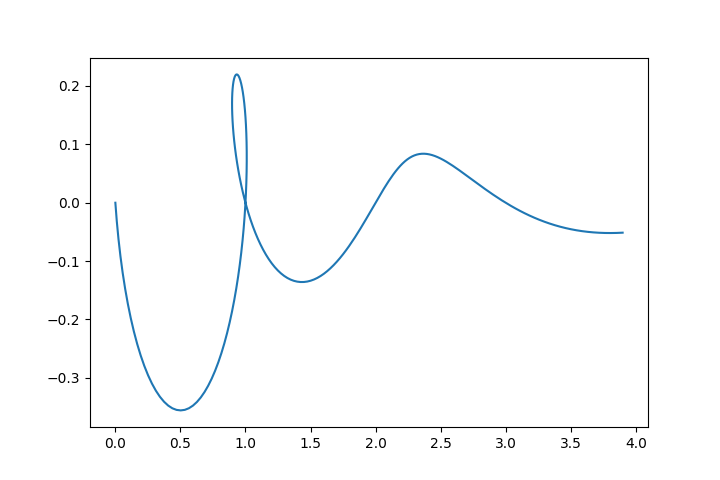
\includegraphics[width=0.5\textwidth]{fibonacci-positive-n.png}

\end{document}
